\subsection{符号说明}

\begin{center}
    \begin{tabularx}{0.8\textwidth}{c@{\hspace{1pc}}|@{\hspace{2pc}}>{\centering\arraybackslash}X}
        \Xhline{0.08em} % 表格顶部粗线
        \textbf{符号} & \textbf{符号说明}            \\
        \Xhline{0.05em}
        $R_i$       & 第 $i$ 个样本“染色体的非整倍体”的检测结果 \\
        $P_i$       & 第 $i$ 个样本预测的“胎儿是否健康”结果   \\
        $H_i$       & 第 $i$ 个样本“胎儿是否健康”的实际情况记录 \\
        $E_i$       & 对第 $i$ 个样本预测准确性的最终评估结果   \\
        \Xhline{0.08em}
    \end{tabularx}
\end{center}

本文建立了评估结果指标 $E_i$ 通过比较预测值 $P_i$ 和实际值 $H_i$ 来确定。如果两者相等，则评估为“准确”；如果不相等，则为“不准确”。
本文可以用一个决策函数来表示：
\begin{equation}
    P_i =
    \begin{cases}
        1 & ,R_i \text{为空} \\
        0 & ,R_i \text{非空}
    \end{cases}
    \quad \quad
    H_i =
    \begin{cases}
        1 & ,\text{“是”} \\
        0 & ,\text{“否”}
    \end{cases}
    \quad \quad
    E_i =
    \begin{cases}
        1 & ,P_i = H_i    \\
        0 & ,P_i \neq H_i
    \end{cases}
\end{equation}

\begin{center}
    \begin{tabularx}{0.8\textwidth}{c@{\hspace{1pc}}|@{\hspace{2pc}}>{\centering\arraybackslash}X}
        \Xhline{0.08em} % 表格顶部粗线
        \textbf{符号}  & \textbf{符号说明（续表）}                                                \\
        \Xhline{0.05em}
        $B$          & BMI分组的边界点向量                                                      \\
        $R(w)$       & 孕周为 $w$ 时的潜在风险函数                                                 \\
        $S_j$        & 第 $j$ 组 ($G_j$) 内的样本集合                                           \\
        $S_{j,w}$    & 第 $j$ 组在孕周窗口 $[w, w+1)$ 内的样本子集                                   \\
        $N_{j,w}$    & 窗口样本数, 即 $|S_{j,w}|$                                             \\
        $A(S_{j,w})$ & 窗口 $S_{j,w}$ 内的检测成功率                                             \\
        $w_j^*$      & 第 $j$ 组的最佳NIPT时点 (孕周)\footnote{在优化理论中，上标星号（*）通常用来表示最优解。另外的符号同理。} \\
        \Xhline{0.08em}
    \end{tabularx}
\end{center}

\subsection{模型假设}

基于题干对探究 BMI 范围与 NIPT 检测时点的关系的要求，本文做出以下假设：

\begin{enumerate}
    \item 假设孕妇的BMI是影响胎儿Y染色体浓度达标时间的主要因素，其他因素可暂时视为次要影响或随机扰动。
    \item 假设风险与孕周的阶梯关系可量化，且风险值随孕周增加而递增。
\end{enumerate}

\subsection{数据分析}

由于男胎的 Y 染色体浓度达到或高于 4\% 才被认为 NIPT 的结果是基本正确的，为了给出每组的 BMI 区间和最佳 NIPT
时点，本文在进行求解前，探究了对男胎孕妇 BMI 与孕周数之间的关系，Y 染色体浓度小于 4\% 的散点被标注出来。同时，孕妇代码 A160 的 BMI 值偏低（$20.7$），视作离群点，不具统计意义，剔除后，分布如图 \ref{fig:BMI 与孕周散点图} 所示：

\begin{figure} [H]
    \centering
    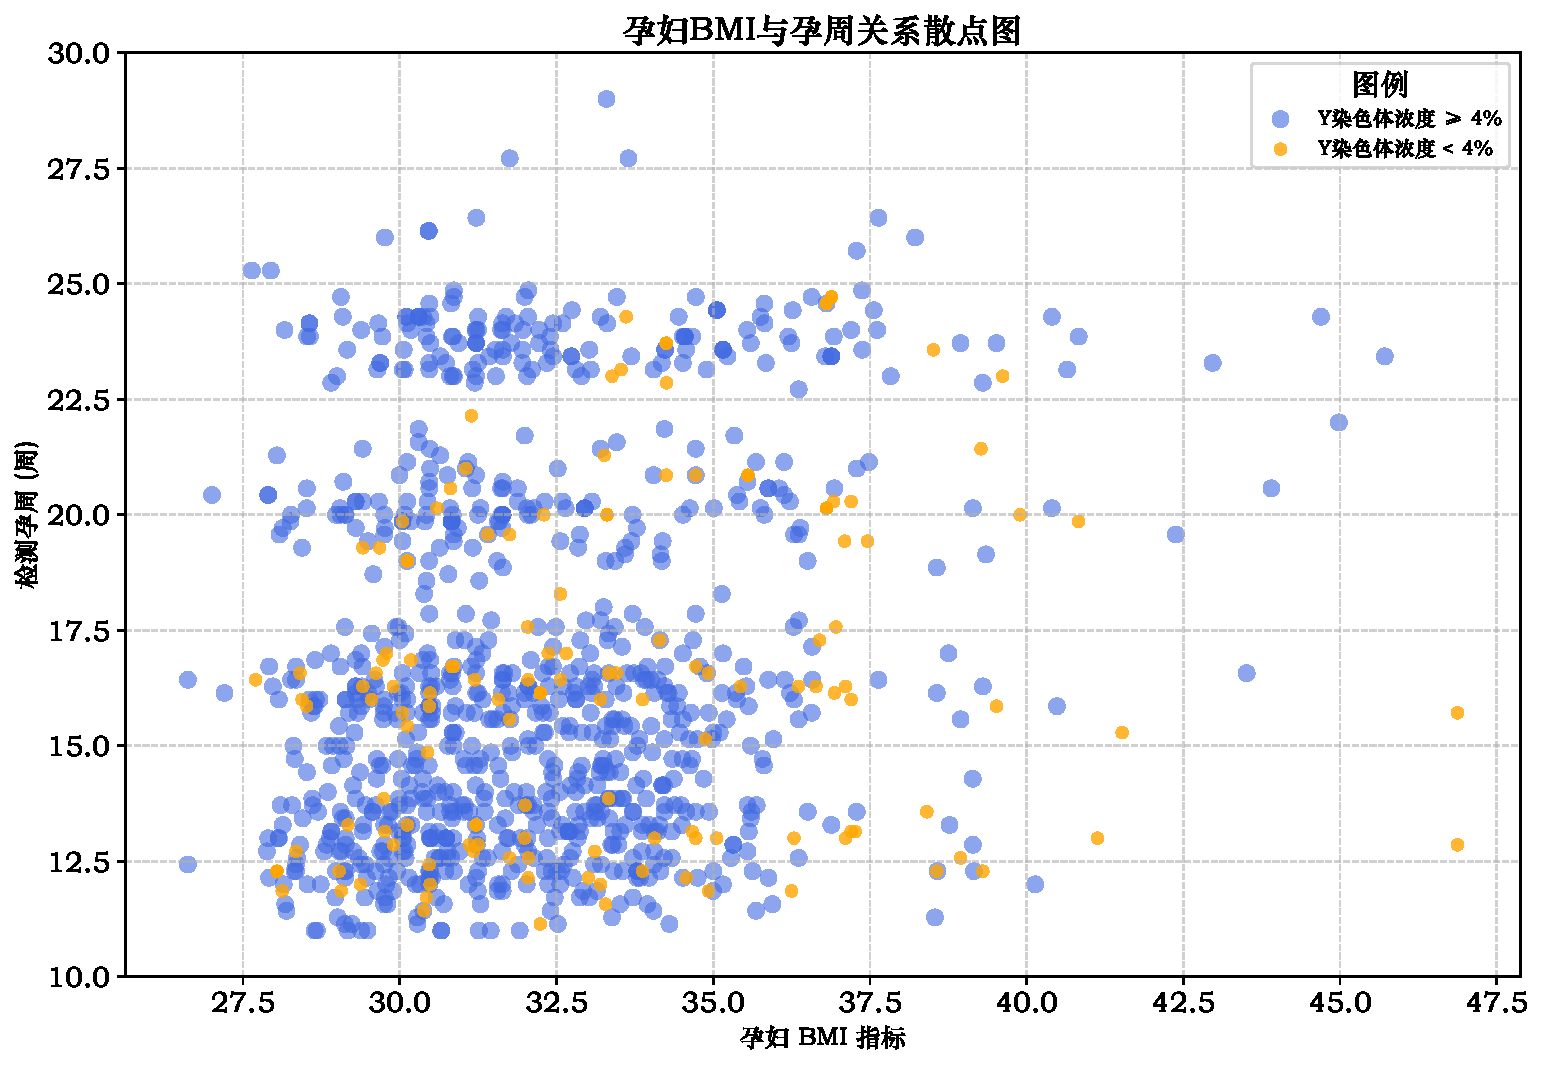
\includegraphics[width=0.7\textwidth]{chapters/Q2/images/BMI 与孕周散点图.pdf}
    \caption{BMI 与孕周散点图}
    \label{fig:BMI 与孕周散点图}
\end{figure}

同时，本文根据上述模型，以红色标注出 NIPT 检验结果不准确的样本（即 $E_i = 0$ 的样本点），分布如图 \ref{fig:检验结果不准确} 所示：

\begin{figure} [H]
    \centering
    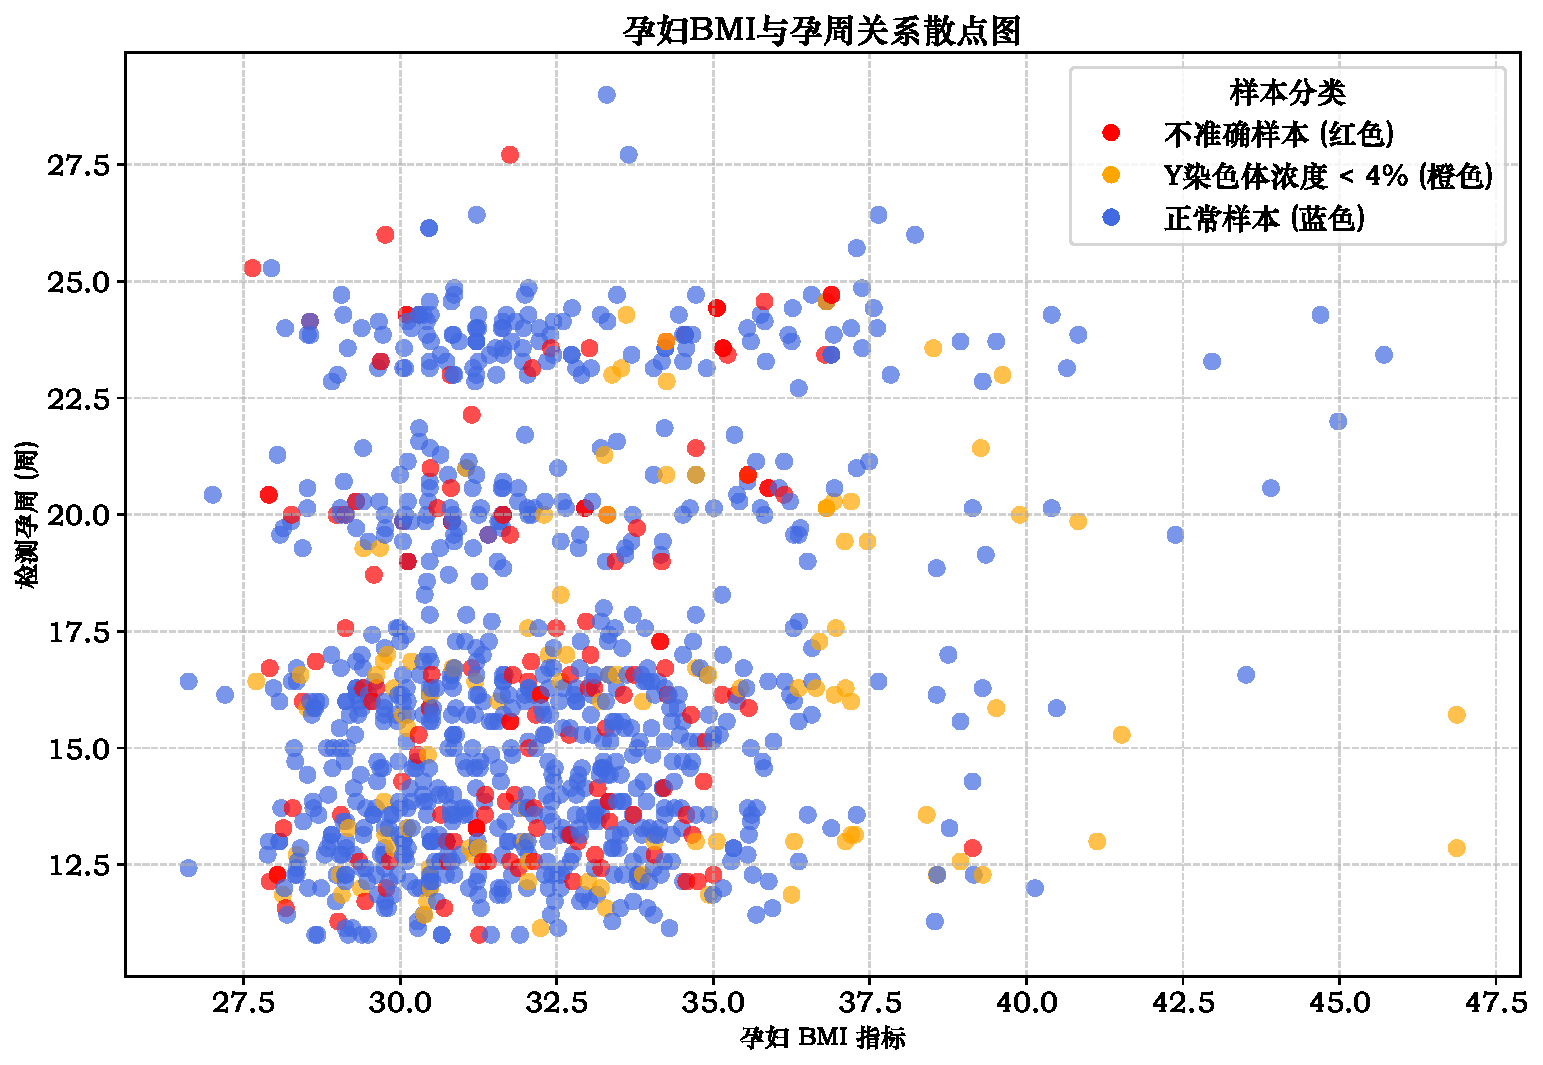
\includegraphics[width=0.7\textwidth]{chapters/Q2/images/标注全部不准确散点图.pdf}
    \caption{检验结果不准确的样本散点图}
    \label{fig:检验结果不准确}
\end{figure}

\subsection{K-Means 算法选择聚类数量}

K-Means 算法预先指定初始聚类数以及初始化聚类中心，按照样本之间的距离大小，把样本集根据数据对象与聚类中心之间的相似度划分为类簇，不断更新聚类中心的位置，不断降低类簇的误差平方和，当 SSE 不再变化或目标函数收敛时，聚类结束，得到最终结果。

\newpage

\begin{enumerate}
    \item 先从数据集中随机选取K个初始聚类中心 $C_j(1 \leq j \leq k)$ ，计算其余数据对象与聚类中心 $C_j$ 的欧氏距离，找出离目标数据对象最近的聚类中心 $C_j$ ，并将数据对象分配到聚类中心 $C_j$ 所对应的簇中；
    \item 接着计算每个簇中数据对象的平均值，将该值当作新的聚类中心，进行下一次迭代，直到聚类中心不再变化或达到最大的迭代次数时停止。
\end{enumerate}

空间中数据对象与聚类中心间的欧氏距离计算公式为：
\begin{equation}
    d\left(X, C_j\right)=\sqrt{\sum_{d=1}^m\left(X_d-C_{j d}\right)^2}
\end{equation}
其中，$X$ 为数据对象；$C_i$ 为第 $i$ 个聚类中心；$m$ 为数据对象的维度；$X_j$、$C_{ij}$ 为 $X$ 和 $C_i$ 的第 $j$ 个属性值。整个数据集的 SSE 计算公式为：
\begin{equation}
    \mathrm{SSE}=\sum_{j=1}^k \sum_{X \in C_j}\left|d\left(X, C_j\right)\right|^2
\end{equation}
其中，SSE 的大小表示聚类结果的好坏；$k$ 为簇的个数。
K-Means 的本质是通过迭代最小化 SSE 实现聚类，默认距离使用欧氏距离。其算法流程图如下所示：
\begin{figure} [H]
    \centering
    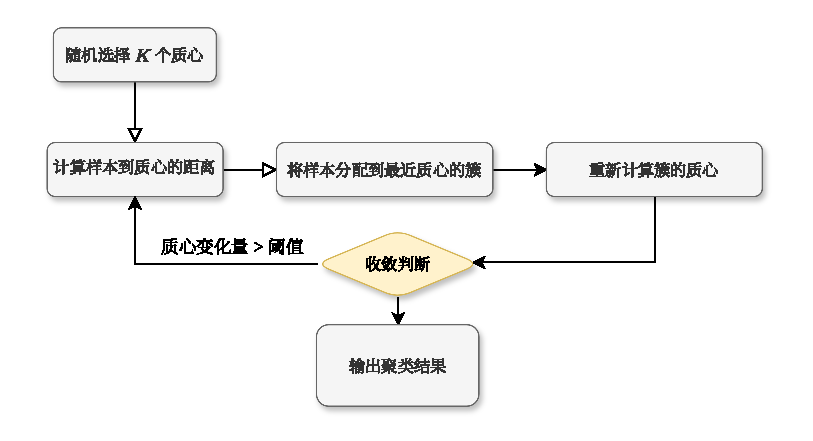
\includegraphics[width=0.65\textwidth]{chapters/Q2/images/KMeans-Drawio.pdf}
    \caption{K-Means 算法流程图}
\end{figure}

本文使用肘部法则确定最优聚类数 $K$。肘部法通过计算不同 $K$ 值下的 SSE，绘制 SSE 随 $K$ 变化的曲线图，选择曲线出现“肘部”位置对应的 $K$ 值作为最优聚类数。绘制的肘部法曲线图如 \ref{fig:K-Means手肘法} 所示。观察图 \ref{fig:K-Means手肘法} 可知，当 $k = 2,3,4$ 时都是可考虑的值。为了让不同 BMI 的孕妇能够获得更精细的 NIPT 检测时点建议，并且也与题干给出的分组组数相似，故本文选择 $k=4$ 作为最终的聚类数。

\begin{figure}[H]
    \centering
    \begin{minipage}{0.48\textwidth}
        \centering
        
\includegraphics[width=\textwidth]{chapters/Q2/images/K-Means手肘法.pdf}
        \caption{K-Means手肘法}
        \label{fig:K-Means手肘法}
    \end{minipage}
    \hfill
    \begin{minipage}{0.48\textwidth}
        \centering
        
\includegraphics[width=\textwidth]{chapters/Q2/images/BMI聚类分析结果.pdf}
        \caption{BMI聚类分析结果}
        \label{fig:BMI聚类分析结果}
    \end{minipage}
\end{figure}

图 \ref{fig:BMI聚类分析结果} 展示了散点图的聚类结果，并且用红线标注了聚类的中心点，从中本文可以看出，聚类效果较好，且各个簇之间的间隔较大，说明不同 BMI 的孕妇在 NIPT 检测时点上可能存在显著差异。

\subsection{多目标优化}

\subsubsection{潜在风险函数}

据题意，本文将不同孕周的潜在风险定义为一个分段函数。早期（$12$周及以内）风险低；中期（$13 \sim 27$周）风险随孕周线性增高；晚期（$28$周及以后）风险极高。具体函数如下：
\begin{equation}
    R(w) =
    \begin{cases}
        1                      & ,\text{若}\ \ w \le 12        \\
        10 + 3 \times (w - 13) & ,\text{若}\ \ 13 \le w \le 27 \\
        100                    & ,\text{若}\ \ w \ge 28
    \end{cases}
    \label{eq:risk_function}
\end{equation}

\subsubsection{加权和法确定目标函数}

寻找最佳的 BMI 区间的核心目标是最小化孕妇的潜在风险，同时最大化采样检测的准确率。通过加权和法，本文将此多目标问题转化为单目标优化问题。目标是寻找一组最优的 BMI 边界点 $B^*$，使得加权的总体目标函数 $F(B)$ 最小。
\begin{equation}
    B^* = \arg\min_{B} F(B)
    \label{eq:optimization_goal}
\end{equation}

\paragraph*{最小化总体潜在风险}

第一个目标是使所有孕妇的平均潜在风险最低。对于一组给定的BMI边界点 $B$，本文可以为每个分组 $G_i$ 找到其最佳检测孕周 $w_i^*$。该分组内所有样本的风险均按 $R(w_i^*)$ 计算。因此，全体样本的加权平均风险 $F_{risk}(B)$ 可以表示为：
\begin{equation}
    \min F_{risk}(B) = \min \left( \frac{\sum_{j=1}^{4} |S_j| \cdot R(w_j^*)}{\sum_{j=1}^{4} |S_j|} \right)
    \label{eq:risk_objective}
\end{equation}
其中 $|S_i|$ 是第 $i$ 组的样本总数，作为权重，以确保样本量大的分组在总体风险评估中占有相应比重。

\paragraph*{最大化总体检测准确率}

第二个目标是使在推荐窗口内进行检测的样本，其总体准确率最高。准确率 $A(S_{i, w_i^*})$ 定义为在第 $i$ 组的最佳窗口 $S_{i, w_i^*}$ 内，检测成功（Y染色体浓度达标且结果准确）的样本比例。总体加权平均准确率 $F_{acc}(B)$ 可以表示为：
\begin{equation}
    \max F_{acc}(B) = \max \left( \frac{\sum_{j=1}^{4} |S_{j, w_j^*}| \cdot A(S_{j, w_j^*})}{\sum_{j=1}^{4} |S_{j, w_j^*}|} \right)
    \label{eq:accuracy_objective}
\end{equation}
其中 $|S_{j, w_j^*}|$ 是推荐窗口内的样本数，作为权重。

\paragraph*{从多目标优化转为单目标优化}

标准的优化算法通常只能处理单一方向（例如求最小值）的问题。本文选择将所有目标统一为\textbf{最小化}。这是由于 minimize 模块是为最小化定制的。对于``最大化准确率"($F_{acc}$)，本文将其等价于\textbf{最小化不准确率}，即 $1 - F_{acc}$，再使用经典的“加权和法”将这两个最小化目标合并为一个单一的、综合的函数 $F(B)$。通过为每个目标分配一个权重（$w_{risk}$ 和 $w_{acc}$），以确保潜在风险最小为首要任务，可人工赋予权重 $w_{risk} = 0.7 > w_{acc} = 0.3$。最终的优化目标可以表示为：
\begin{equation}
    B^* = \arg\min_{B} F(B)
    \label{eq:optimization_goal}
\end{equation}
其中，总体目标函数 $F(B)$ 定义为所有分组的加权风险与加权不准确率之和：
\begin{equation}
    F(B) = w_{risk} \cdot F_{risk}(B) + w_{acc} \cdot \left( 1 - F_{acc}(B) \right)
    \label{eq:objective_function_final}
\end{equation}

\subsubsection{约束条件}

为了确保模型解的合理性和统计有效性，优化过程必须满足以下约束条件：

\begin{enumerate}
    \item \textbf{边界点单调性}: 为了保证BMI分组的逻辑正确性，分为四组需 5个边界点 $b_i$，满足单调递增关系，即 $b_i < b_{i+1}$，其中 $i = 1, 2, 3, 4$。

    \item \textbf{推荐窗口宽度}: 考虑到临床操作的灵活性和单周样本量的稀疏性问题，本文将NIPT推荐时间窗口的宽度设定为\textbf{两周}。例如，若推荐起始周为 $w_i^*$，则对应的窗口为 $[w_i^*, w_i^*+2)$。

    \item \textbf{窗口样本量约束}: 为了保证所选窗口的成功率计算具有统计学意义，同时避免结果被样本量异常集中的窗口所主导，本文对窗口内的样本数量 $N_{j, w_j^*}$ 设定了上下限。在本模型中，本文设定最小样本数为 $50$，最大样本数为 $100$。
          \begin{equation}
              50 \le N_{j, w_j^*} = |S_{j, w_j^*}| \le 100, \quad \forall j \in \{1, 2, 3, 4\}
              \label{eq:constraint_new}
          \end{equation}
\end{enumerate}

本文采用 Python 中的 scipy.optimize.minimize 库，基于序列最小二乘规划（SLSQP）求解器对目标函数进行迭代优化，寻找最优的 BMI 边界点。
为了提高优化效率，使用 BMI 的 $0, 25, 50, 75, 100$ 百分位点作为初始边界点（如图 \ref{fig:BMI四分位点}）。

\begin{figure} [H]
    \centering
    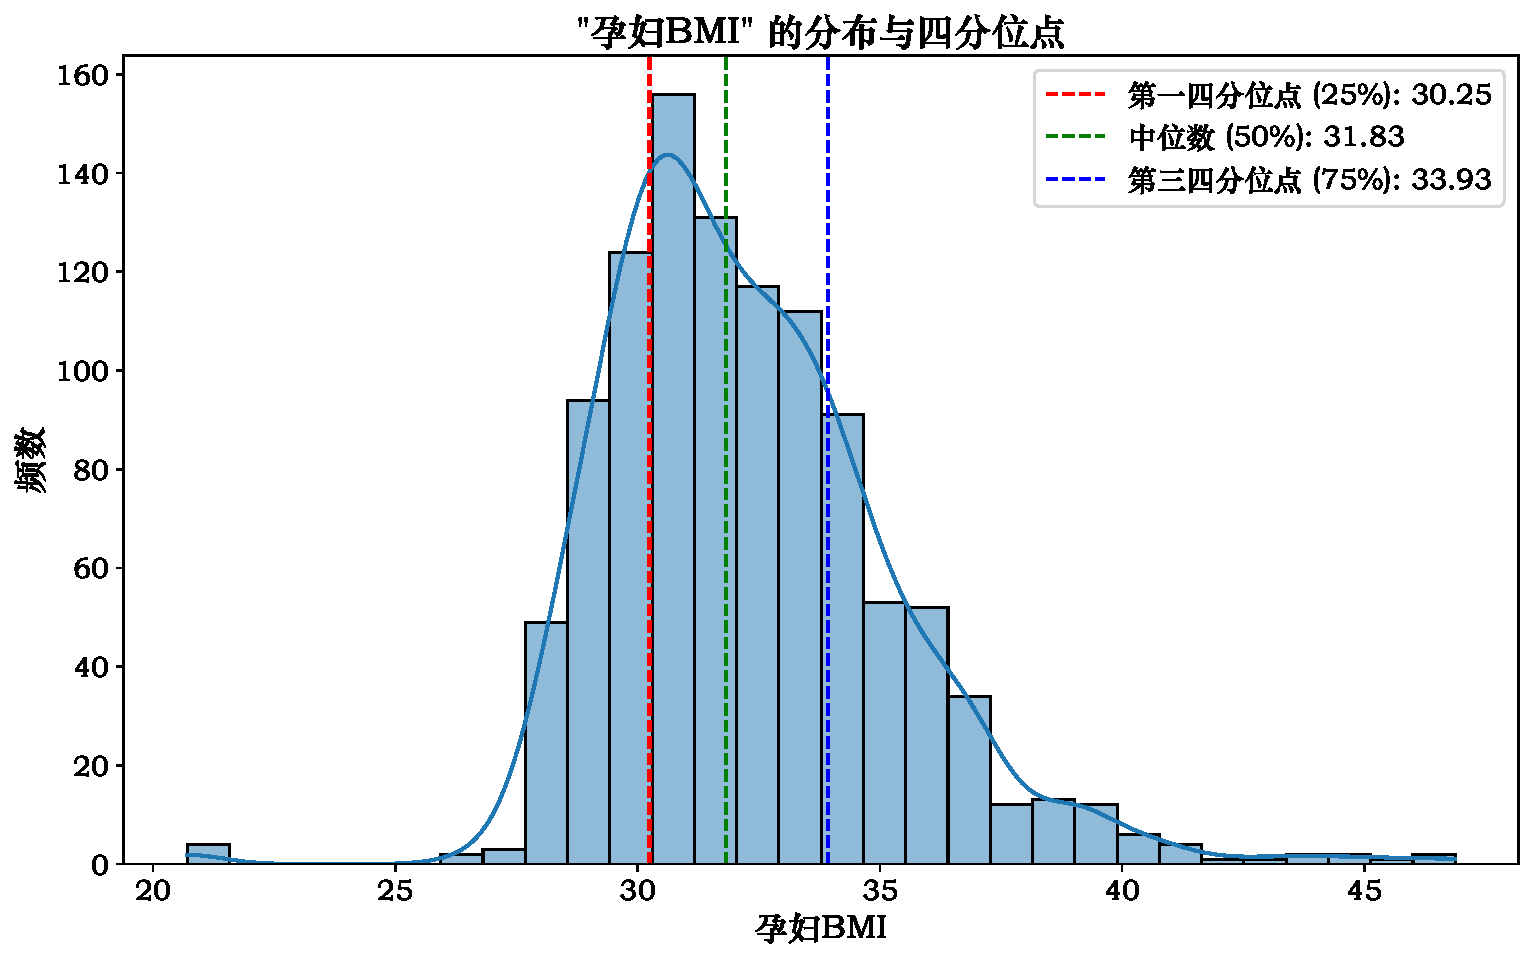
\includegraphics[width=0.6\textwidth]{chapters/Q2/images/孕妇BMI的四分位点.pdf}
    \caption{孕妇BMI的四分位点}
    \label{fig:BMI四分位点}
\end{figure}

经优化，本文得到的最优 BMI 分组方案及对应的最佳 NIPT 时点建议如表 \ref{tab:results} 所示。

\begin{table}[H]
    \centering
    \caption{最优BMI分组及NIPT时点推荐方案}
    \label{tab:results}
    \begin{tabular}{ccccc}
        \toprule
        \textbf{BMI分组} & \textbf{BMI区间} & \textbf{最佳NIPT时点 (周)} & \textbf{窗口内样本数} & \textbf{窗口内成功率} \\
        \midrule
        分组 1           & [26.62, 30.28) & 13 -- 15              & 60              & 85.00\%         \\
        分组 2           & [30.28, 31.88) & 15 -- 17              & 58              & 77.59\%         \\
        分组 3           & [31.88, 33.95) & 14 -- 16              & 52              & 90.38\%         \\
        分组 4           & [33.95, 46.87) & 15 -- 17              & 59              & 69.49\%         \\
        \bottomrule
    \end{tabular}
\end{table}

\v{-1em}

为直观验证上述优化方案的有效性，本文将表 \ref{tab:results} 中得到的四个最优 NIPT 推荐窗口，以高亮矩形区域的形式叠加绘制在原始的散点图上，结果如 \ref{fig:BMI分组和最佳NIPT时点} 所示。推荐窗口精确地覆盖了正常样本（蓝色点）的密集区域，同时有效规避了不准确样本（红色点）和Y染色体浓度过低样本（橙色点）的集中分布区。这种直观的对应关系，证实了该模型在平衡检测成功率与潜在风险两方面的优越性。

\begin{figure} [H]
    \centering
    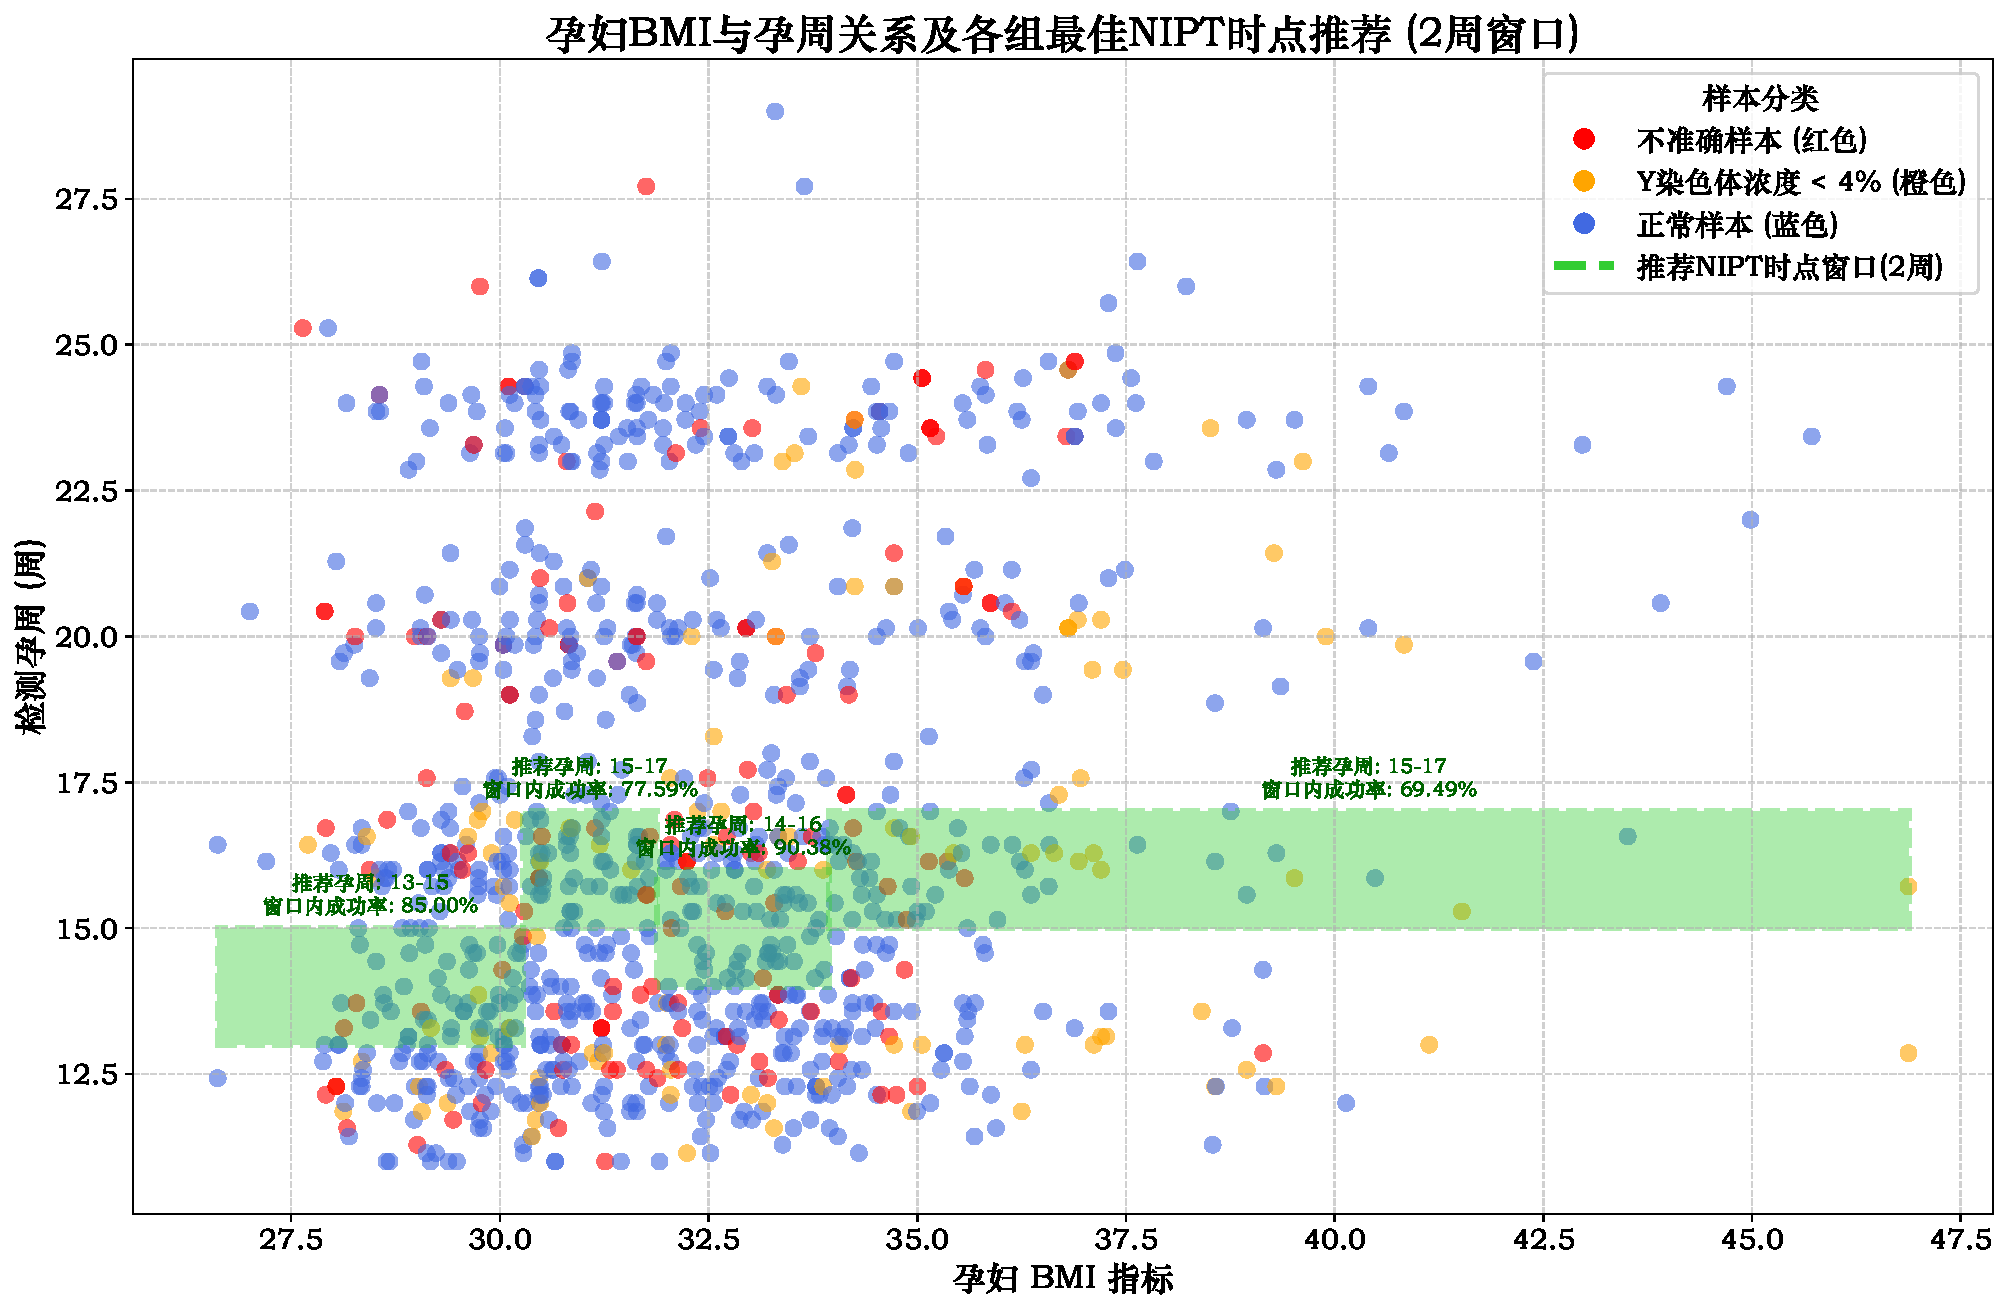
\includegraphics[width=0.75\textwidth]{chapters/Q2/images/BMI分组和最佳NIPT时点.pdf}
    \caption{BMI分组和最佳NIPT时点}
    \label{fig:BMI分组和最佳NIPT时点}
\end{figure}

表 \ref{tab:results} 将孕妇 BMI 值划分为四个亚组，其合理性在于借鉴了临床通用的 BMI 四分类标准（偏瘦、正常、超重、肥胖）思想\cite{WHO2005SuRF}，实现了对高风险人群的内部精细化分层。孕期母体为支持胎儿生长、胎盘发育及增加血容量等生理需求，体重和 BMI 必然显著增加\cite{kominiarek2017gestational}。该方案为不同 BMI 区间的孕妇提供了精确、可靠的 NIPT 检测时间窗口建议。所有推荐窗口均基于超过 $50$ 个样本的数据得出，保证了结论的统计稳健性。不仅如此，通过敏感性分析证实，当模型中的权重系数在 20\% 的容差范围内浮动时，最终得出的最优分组方案与时点建议均保持不变，充分证明了该决策模型的参数稳健性。由于过高或过低的 BMI 样本较少，本文模仿四分类标准，为男胎孕妇提供更具普适性的 BMI 与 NIPT 检测时间窗口建议（于表 \ref{tab:optimized_nipt_schedule}）。

\begin{table}[H]
    \centering
    \caption{基于BMI分层的NIPT最佳时点推荐方案}
    \label{tab:optimized_nipt_schedule}
    \begin{tabular}{cc}
        \toprule
        \textbf{BMI范围}           & \textbf{推荐NIPT最佳检测孕周} \\
        \midrule
        $BMI < 30.28$            & $13 \sim 15$ 周        \\
        $30.28 \leq BMI < 31.88$ & $15 \sim 17$ 周        \\
        $31.88 \leq BMI < 33.95$ & $14 \sim 16$ 周        \\
        $33.95 \leq BMI$         & $15 \sim 17$ 周        \\
        \bottomrule
    \end{tabular}
\end{table}

\begin{center}
    \begin{tikzpicture}
        % 绘制带箭头的数轴，并标记为 BMI
        \draw[->, thick] (0,0) -- (12,0) node[right] {BMI};

        % --- 定义关键坐标点 ---
        % 这里我们将 BMI 的范围映射到 x 轴的 0-12 范围内以便于绘图
        \def\pointOne{3.5}   % 对应 BMI 30.28
        \def\pointTwo{6}     % 对应 BMI 31.88
        \def\pointThree{9}   % 对应 BMI 33.95

        % --- 标记数轴上的关键点 ---
        % 绘制小圆点并在线下方标记数值
        \draw (\pointOne, 0) circle (2pt) node[below=4pt] {$30.28$};
        \draw (\pointTwo, 0) circle (2pt) node[below=4pt] {$31.88$};
        \draw (\pointThree, 0) circle (2pt) node[below=4pt] {$33.95$};

        % --- 在数轴上方绘制分段大括号并标注推荐孕周 ---
        % amplitude=10pt 控制了大括号的"胖瘦"，值越大，括号越大
        % above=15pt 控制了括号上方文字的距离
        \draw [decorate, decoration={brace, amplitude=10pt}]
        (0,0) -- (\pointOne,0)
        node [midway, above=15pt] {$13 \sim 15$ 周};

        \draw [decorate, decoration={brace, amplitude=10pt}]
        (\pointOne,0) -- (\pointTwo,0)
        node [midway, above=15pt] {$15 \sim 17$ 周};

        \draw [decorate, decoration={brace, amplitude=10pt}]
        (\pointTwo,0) -- (\pointThree,0)
        node [midway, above=15pt] {$14 \sim 16$ 周};

        \draw [decorate, decoration={brace, amplitude=10pt}]
        (\pointThree,0) -- (12,0)
        node [midway, above=15pt] {$15 \sim 17$ 周};

    \end{tikzpicture}
\end{center}

为探究孕妇 BMI 对所需孕周 $w$ 的影响，本文据问题一中构建的模型（见式 \ref{eq:final_model}）进行分析。在保持 Y 值与协变量检测次数 $c$ 恒定的条件下，对该式进行移项可得：
\begin{equation}
    Y - 0.218290 - 0.012028c + 0.002045 \cdot BMI = 0.000326w^2 - 0.011993w
\end{equation}

等式左侧是随 BMI 值单调递增的线性函数。为维持等式成立，等式右侧关于 $w$ 的二次函数 $f(w) = 0.000326w^2 - 0.011993w$ 的值也必须相应增大。该二次函数在 $w > 18.39$ 的区间内为增函数，符合本文中 $w$（孕周）的实际取值范围。在其他条件不变时，BMI 越高的孕妇，需要越长的孕周（即越大的 $w$ 值）才能达到相同的 $Y$ 值。BMI 越高的孕妇群体，其 Y 染色体浓度达到 $4\%$ 标准所需的孕周越长（即越大的 $w$ 值），在权衡检测准确度和潜在风险的前提下，建议的 NIPT 时点也相应推迟，与本文表 \ref{tab:optimized_nipt_schedule} 中的高 BMI 推荐最佳检测孕周相对应。

\subsection{模型有效性与检测误差分析}

在本文的数据情境下，“检测误差”由可观测的两种不良检测样本点构成，即检测不准确点（红色）与检测失败点（橙色，男胎Y染色体浓度低于4\%，导致本次检测不可靠）。检测失败常要求孕妇重新检测，增加成本、延长诊断时间，无疑会增加孕妇及其家庭的焦虑，并压缩了后续可能的医疗干预窗口。

为评估本模型规避检测误差的效果，本文采用\textbf{组内对比分析}方法，将当前推荐的最佳NIPT窗口内的成功率，与该分组自身的所有样本的平均成功率进行比较。

\subsubsection{组内成功率对比}

在模型根据全局目标函数（公式 \ref{eq:objective_function_final}）找到最优的BMI边界点后，本文对划分出的四个孕妇群体进行组内分析。详细的对比数据如图 \ref{fig:组内检测成功率对比图} 所示。

\begin{figure} [H]
    \centering
    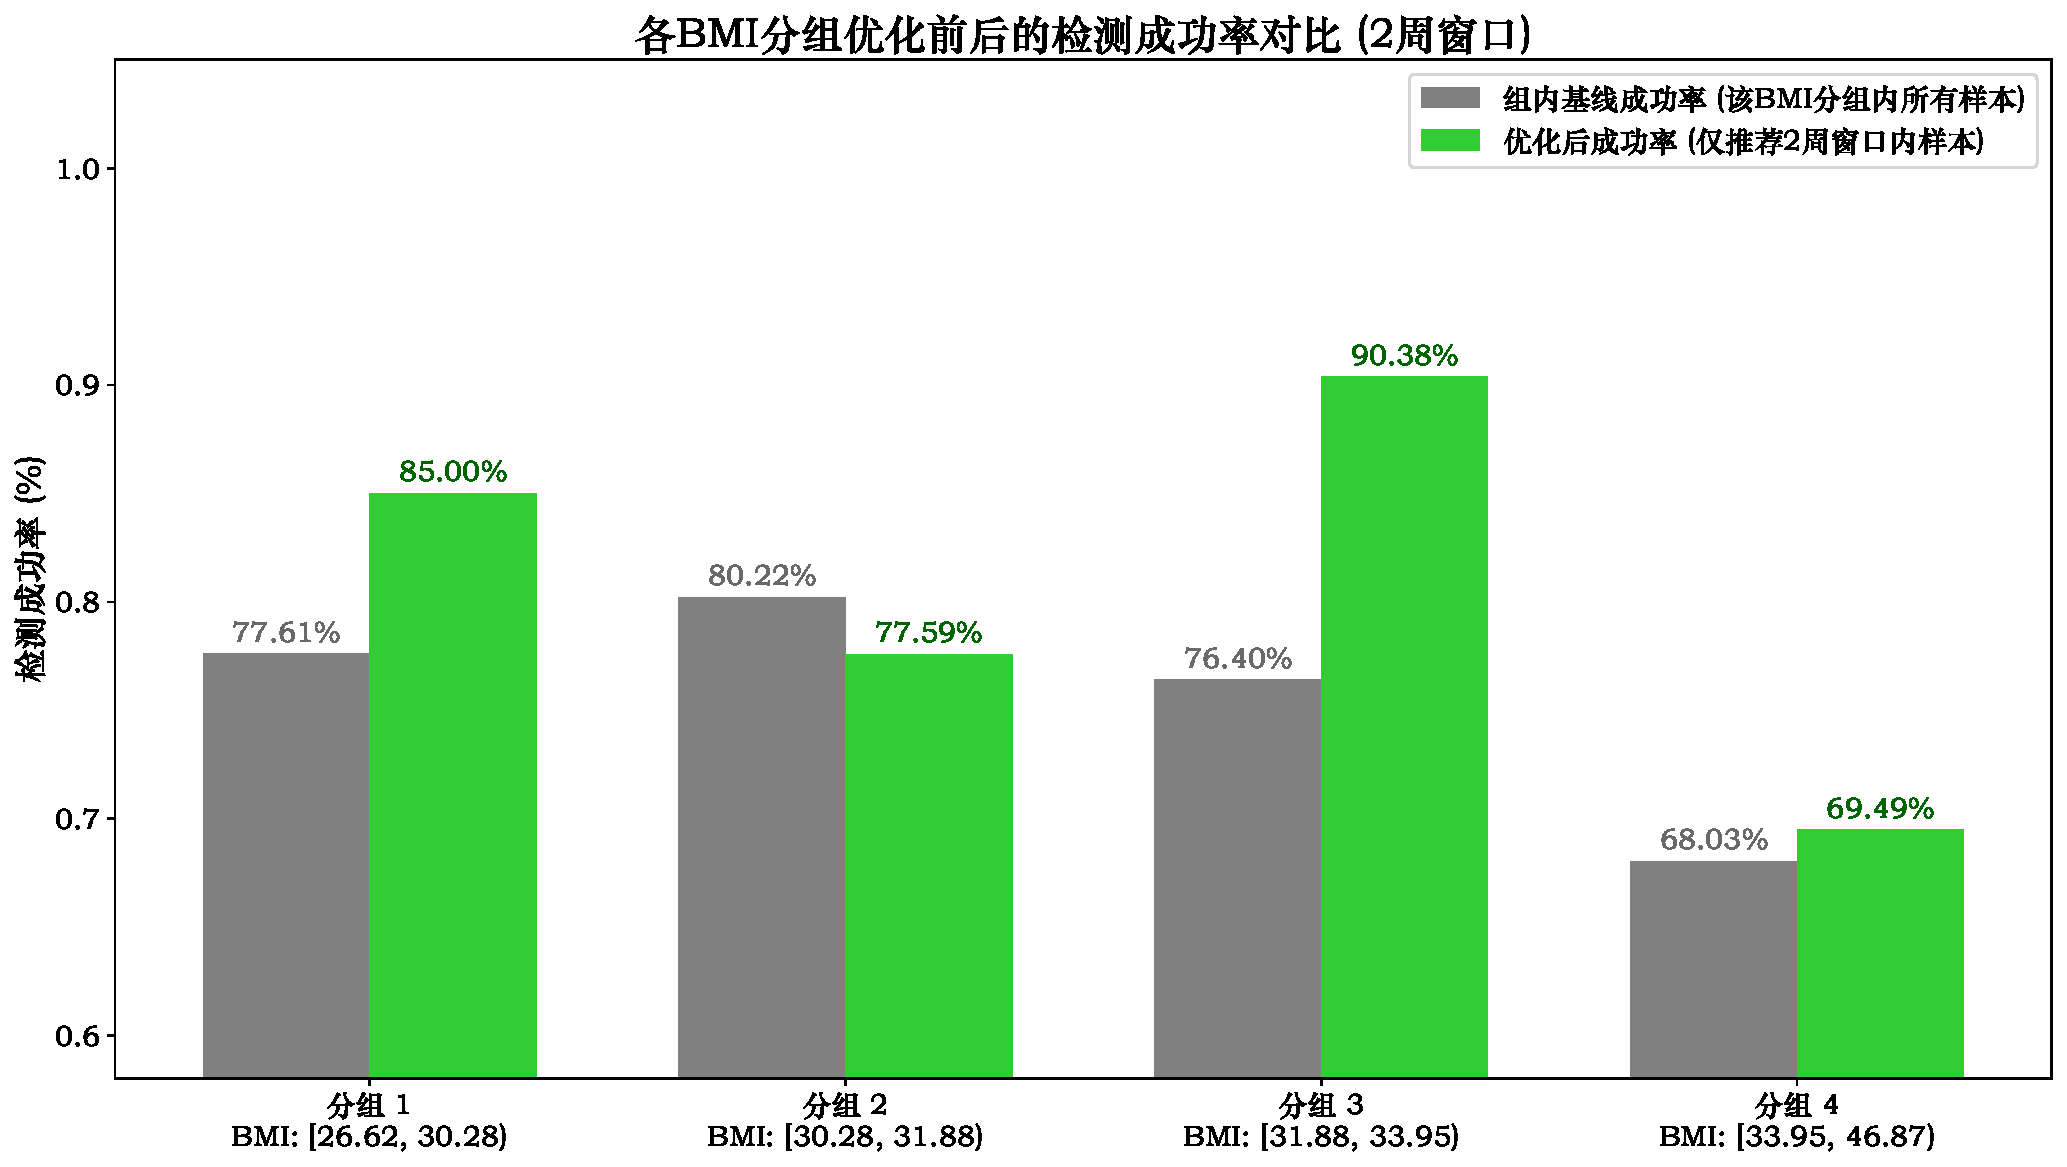
\includegraphics[width=0.8\textwidth]{chapters/Q2/images/组内检测成功率对比分析.pdf}
    \caption{组内检测成功率对比图}
    \label{fig:组内检测成功率对比图}
\end{figure}

对于分组1、3，本模型推荐的NIPT窗口极大地提升了检测成功率，而分组 2 略低于该组的基线水平的原因是模型为降低风险，选择了成功率稍低的窗口，该决策很可能使分组 3 的检测成功率大幅提升。证明了检测误差是塑造最终决策结果的驱动之一。它不仅是模型需要规避的对象，更是迫使模型进行智能权衡的关键因素。
